% ----------------------------------------------------------------------------------------
% CHAPTER TITLE
% ----------------------------------------------------------------------------------------
\chapter{Interviews: highlights and analyses}\label{interviews}
\lhead{\chaptertitlename\ \thechapter. \emph{Interviews}}
% ----------------------------------------------------------------------------------------
This section presents a set of highlights from interviews with current practitioners, most of which were responsible for the projects in chapter three. The goals of these interviews was to expose underlying motivations behind those projects, identify any underlying trends, and give an experiential account of the electronic instrument design community. 

Through their work, these artists and engineers have offered a vision for a fragmented practice united by a common curiosity in the devices that make their music possible. They do not necessarily represent the entire space of possibilities, but rather illustrate that this fragmentation and openness ultimately creates a robust, self-sustaining and multi-faceted space for hardware creation in a musical context.

\section{Methodology}

In the process of preparing interviews, five themes around which to organize questions were chosen. Those were the following: 

\begin{itemize}
	\item current place of hardware in their work 
	\item dealing with technical limitations
	\item their perception of the professional community they might feel part of
	\item the importance of an ethos in their design work
	\item engagement with the questions of experimental or avant-garde music 
	\end{itemize}

These points were then adapted to fit the preliminary research undertaken for each interviewee. They were complemented when necessary by questions regarding each person's background or specific experience. Four exchanges took place over email (Martin Howse, Louise \& Ben Hinz, Bonnie Jones, Jessica Rylan), which was less flexible but offered more time for the responders. The other four took place in person (Nicolas Collins, Sunny Nam, Dan Snazelle) or over the phone (Tristan Shone). All of those interactions happened between November 2014 and March 2015. 

The goal was to get an understanding of their current relations to electronic music hardware, how they developed that approach, and where they see it going next. This section details highlights and analyses derived from this body of statements. Rather than inquiring explicitly about conceptual ideas such as post-optimal objects, more practical topics allowed for concepts to emerge by themselves when the interviewee wished to discuss them.  

\emph{Please refer to appendix A for full transcripts. Unless explicitly noted, all quotes within a section are from the interviewee for that section.}
	
\section{Louise and Ben Hinz}

Louise and Ben Hinz are self-taught inventors who have professionalized an interest in musical tinkering and are now both professional ``silicon luthiers''. Interviewing them was an opportunity to discuss their path and see if any element of their methodology fit within a post-optimal approach to electronic audio hardware. 

\begin{quote}
	We bought about \$40 worth of parts, a soldering iron and a book on hardware hacking. He had no background in electronics at all. He just kept reading and trying stuff out until he understood it.
\end{quote}

In this learning process (the book they mention was of course \citep{collins2006}), the Hinz would come to develop an appreciation for the unexpected mistake, but also for the power of cleverly-arranged simplicity:  

\begin{quote}
	
	Some of my early work came from using components incorrectly to get weird sounds that were not available elsewhere, which is still really important to us. We decided a few years ago that if we couldn’t do something new and interesting that we loved, we wouldn’t do it at all. (...) for the most part I just apply fairly common knowledge in unconventional ways, so I wouldn’t really be blowing anyone’s hair back.
	
	\end{quote}

Their re-use of ``common knowledge in unconventional ways'' brings up the issue of ownership in audio circuit design. Legally, a copyright only protects the raw schematic circuit representation and does not prevent others from producing minor variations of that schematic or of the circuit it describes. In the United States, legal protection from copies can only be achieved through much more difficultly obtained patents, which most designers rarely attempt to get. Music technology is a rare case in which copyright law effectively encourages copies. 

The Hinz' financial success can therefore be attributed to the build quality and variety of their work. Dwarfcraft Devices has recently released their first digital product, the \textit{Pitchgrinder}:  

\begin{quote}
	
Digital is the future. It's also the now. Most of the ideas I currently have could only be realized digitally. I think there are tons of great analog circuits, and I will use them forever, but for me I'm much more interested in pursuing digital audio processing. We got started on the Pitchgrinder when I was introduced to Bob Lowe, an engineer here in Eau Claire. I threw a boatload of ideas at him, and we kind of sussed out what was doable from there.
\end{quote}

Elaborating on their general design methods, Ben adds that this back and forth between tinkerer and engineer
 	has become an important aspect of their process: 

\begin{quote}
 	Usually I ask for EVERYTHING. Then I see how many “Nos” and “Maybes” I get back from our engineers (myself included) and usually I try to figure out at least one of the “Nos” and often times we can cram in a couple “maybes” too. Better to go for it all and whittle it down than start small and realize what you could have done far better after the fucking thing is in stores. The same with recording, actually. “Can I put another drum track on there?” “Hell yeah, I already did 12 guitars, we’ll whittle it down later.”
 \end{quote}
 
Beyond the connection he makes between recording and product design, these statements are relevant because they suggest that post-optimal approaches to audio electronics are complementary to classic engineering methodology rather than contradictory. This is doubly verified when Ben also suggests the relevance of others in their technical work: 

\begin{quote}
	Very important now. Early on, I did all of the designs myself and just paid someone else to lay out the PCB for us. The things we’re working on at the moment are collaborative, but mostly they stem from my ideas, and I guide the design process. It’s far better to hire someone who has the skills I don’t, rather than try to master EVERYTHING, and end up losing my shit in the process. We have one full time “techinical” Henchman in the workshop, and Bob Lowe works in his own shop, on his own time.
\end{quote}

In effect, post-optimal approaches to silicon luthiery benefit not only from the variety of electronic parts and materials made available through mass-market product manufacture, but also from that very same manufacturing structure. 

\section{Bonnie Jones}

Bonnie Jones was of interest to this project because she has performed extensively using a set of live-bended digital delays and an assorted set of complementary systems (some of which quite Tudor-like in their indeterminacy). Live circuit bending is done by exposing the circuit board of guitar effects and creating momentary shorts within and between devices. 

\begin{figure}[hbt]
  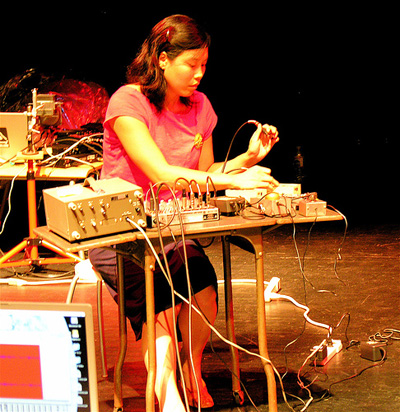
\includegraphics{bonnie}
  \caption{Bonnie Jones performing with a live circuit bending setup. courtesy of simple geometry records}
\end{figure}

Furthermore, her experience founding, directing and teaching for Techne (an electronic music hardware summer program for girls \citep{techne}) placed her in a privileged position to discuss making and composing as it relates to gender and education. 

Let us focus first on Jones' primary instrument, the delay pedal. As she details, an element that is often used to make up a shortcoming of electric instruments — their temporal flatness, the lack of space-related delays — is turned into an instrument by the charged process of turning it upside down and opening it, exposing the circuit board and making it as much of tactile instrument as a ``sax, or a violin'':  live circuit bending can be a valid and respected instance of instrumentation. 

Delay pedals are not meant to be opened and played by touching wires to the circuit board as Jones does. In that sense, she exposes an immediate and potentially universal approach to making an electronic object post-optimal. By connecting elements of a circuit within or between devices, she is blurring the lines between system and interface through a component with unique agency: herself. She resumes that exploration as such: 

\begin{quote}
	I like to say that my set up came about like discovering a language written on a cave wall. As a musician I always approached playing as a way to understand the basic structure of that language as well as the process I can use to learn how to communicate with that language. I suppose the word that could be used is an intuitive approach to understanding the technical aspects of my instruments and their musical possibility.
\end{quote}

Relating to Tudor's vision of indeterminacy, Jones' approach to unpredictable behaviors is explicitly rooted in practice and expertise. ``I appreciate when that instrument has surprises or enables me to create sounds that I wouldn't expect''. However, all efforts ultimately need to be justified: ``I wouldn't care if something was complex if I didn't like the way it sounded.'' This practical approach reflects that of Shone, or Snazelle. Introducing context-specific elements or free software tools in her performance allows her to respond to a particular prompt, and possibly to engage more closely with the audience. This emphasis on the responsibility of the author to cater to a public seems specific to a set of performative traditions, with a care for transparency. This is confirmed by her activities with Techne: 

\begin{quote}
	I take the approach where teaching and working with my nonprofit TECHNE is part of the continuum of my entire creative practice. It’s been important and freeing to unbox the areas of my life that would seem disparate and try to get around the cause/effect/influence categorization.
\end{quote}

The cultural and social connections between audio hardware and communities is once more made explicit. In this case, Jones sees a clear purpose for DIY culture: 

\begin{quote}
	I still see DIY culture as pretty critical. Even in its co-opted and packaged state, being able to make shit with whatever is available to you is pure improvisation. I appreciate that and seek that out. (...) the technological arms race in the arts is tricky. Artist as R\&D for technology corporations is a real thing. Subversion is still the place where those other voices can be heard. (...) I still believe that the most radical shifts happen when artists without the benefit of institutional, financial, or technological supports, just make things happen.
\end{quote}

The latter point relates to the analysis presented in the historical background section, which showed that electronic music hardware went through cycles of institutionalization and democratization. By explicitly noting the lineage of her practice within this history of self-supporting tinkerers, she appears as a particularly legitimate teacher and mentor. 

Jones concludes her answers with the following statement:  

\begin{quote}
The object has a life – the object pushes you and you push it. You can make things that you do not understand at all and maybe later you figure it out and maybe not. Abstraction and improvisation is about hiding and revealing the self at the same time – because of that it is also about resistance. I care about communication but there are so many ways to communicate and so many languages in which to do that.

I am deeply skeptical and suspicious of what is visible.	
\end{quote}

Jones' hardware emphasizes post-optimal possibilities within commercialized items, and her teaching expresses a clear appreciation for a strong and supportive community within the arts. However, she is unique through her experience as a writer and installation artist: those activities conferring a unique sense of self on her artistic perspective. 

\section{Jessica Rylan}

Jessica Rylan was included here for her interest in chaotic / semi autonomous systems in composition. In her discussion with Tara Rodgers, she expressed a disappointment in standard paradigms for audio synthesis, and in the biased communities of the musical electronics field \citep{rodgers2010}. She's currently pursuing nano-optics research at Stanford, meaning that her audio hardware design and performances have slowed to a standstill. However, getting a chance to have her elaborate on some of those topics was a good opportunity to discuss some her previous claims and interests. 

In her replies, self-limitations such as not using an oscilloscope / multimeter for a year, or picking the circuit based on how its schematic looks rather than how it sounds offer a clear post-optimal alternative to regular product design. Her scientific progression is particularly relevant in understanding this methodology: periods of self-teaching and experimentation followed by intense involvement in academic environments, a period as a employee of Don Buchla's business, and finally a relative abandon of the musical world for doctoral scientific research  

She addresses the issue developed by Collins of the engineer which is not the best player of its own designs, saying ``I found design to be a really exciting world for discovering sounds I hadn't heard before and didn't know existed, as well as a way to realize sounds I wanted to hear but couldn't find.''

Rylan's main implementation in a performance context was the \textit{Personal Synthesizer}, presented in section 3.2.1 as a unusual implementation of circuits, with its unpredictable output making it have post-optimal design characteristics. This, once more, brings us back to the post-optimal concept of musical chaos. Rylan presents chaos as inherently more musically interesting in the analog domain: 

\begin{quote}
	the dynamic range limitation in an analog circuit causes limit cycles in chaotic behavior, but this is a generally good thing for music. Moreover, the many noise sources in analog circuits, which operate over many different time scales, help chaotic analog circuits sound good. That noise is entirely absent in digital instruments, unless it is specifically added in. But the main killer is that even in this day and age, digital “chaos” is rarely real-time. Even a modern laptop only has four FPU’s, and they can only do so much. Analog is always real-time, 100\% of the time. I’ll put it specifically: I have never in my life heard a laptop performer get the beautiful chuffing/breathing sound that I sometimes am lucky enough to find with analog circuits in feedback loops.
\end{quote}

Another point that resonates strongly is the relationship between her academic experience and her musical experiments: ``the approach to circuit design taught in engineering programs is strictly at odds with the kind of music that the personal synth allowed for.'' As Collins described in his interviewee (section 4.6), Tudor was uncomfortable with electronics until Mumma gave up on teaching him vacuum tube circuit design and moved to solid state devices. The lesson here seems to be that successfully combining both practices is based mostly on a fragile balance between intuition and curiosity, with both depending on finding the right type of medium. The fantasies that Rylan expresses a few lines later - daydreaming of ``having our own fab and making our own transistors,'' appears as typical of the grandiose ideas that often fuel simpler projects, as well as what we can ultimately hope for from developments in open design and fabrication. She however was probably the most skeptical of the interviewees when it came to discussing the potential of open information on circuits empowering musicians: 

\begin{quote}
	I doubt that designing the instrument yourself necessarily means that relationship is “deeper” somehow, since there are a lot of engineers who are music fans but terrible musicians, and a lot of sound artists who are terrible circuit designers. (...) Of all the people who embark on building electronics specifically for music, very few end up building anything more complicated than a square wave oscillator, and a tiny tiny fraction of those people learn to understand circuits and design their own instruments. Perhaps this sounds elitist but it’s just true. It has actually been a source of great sadness for me, because as much as I enjoyed leading hands-on electronics workshops, I ultimately came to question their value. The learning curve in electronics is very difficult.
\end{quote}

Her opinion on community is along similar pessimistic lines, addressing the under-discussed issue of gender balance in this field: 

\begin{quote}
	There were only a few people who I ever really discussed circuit design with. It would have been nice to know more people, but it’s a very small community and widely dispersed geographically. Also, all men, which definitely effects the social dynamic.
\end{quote} 

On this final point, the field of electronic music is purely sub-optimal. 

Rylan ultimately seems to be one of the best-informed people when it comes to musical applications of engineering concepts. Through that knowledge, she's assembled one of the most compelling example of alternative musical electronics which exhibit a number of post-optimal design decisions matching Dunne's description, however, it also seems to have also justified a clear disinterest in digital implementations of musical chaos, when other interviewees did not have such strong opinions on the matter. 

\section{Dan Snazelle}

Dan Snazelle was interviewed because of his work with the Ardcore synthesizer module, which effectively brings a tradition of additive and subtractive synthesis with the multipurpose paradigms of more recent microprocessor-based synthesis. As research revealed that this project was a collaboration between Snazelle and Darwin Grosse, the set of questions prepared for Snazelle also attempted to get more information concerning this collaborative, hybrid system in electronic music. It also inquired about the development of a small community around the Ardcore's collaborative and open code base. 

Snazelle's initial commercial line marketed in 2007 under the Snazzy FX label consisted of three guitar pedals. This isn't due to a particular interest in the format. Rather, at his company's beginning, the boutique synthesizer module market was a small one and guitar pedals would be easier to sell without needing significant design changes. 

The connection between DIY, guitar electronics, and more standalone synthesis hardware is important, reminiscent of the Hinz' current trajectory. Pedals offer a first, simple practical experience for many musicians, especially those coming from a popular music context rather than an experimental, avant-garde or contemporary classical one. The relatively low complexity means that the high barrier set by engineering described by Jessica Rylan can appear less insurmountable, and successful professional careers can be built around those efforts. 

Furthermore, pedals' simplicity can beat that of even the simplest digital circuits. Snazelle is only one of many practitioners who feel like analog operates on a more human and approachable scale, which often results in an intuitive connection to analog-centric systems (even with modular synthesizers becoming increasingly digital). Regardless of the initial or current complexity, his design methodology has remained consistent: 

\begin{quote}
	I guess I try to think on a systems level, with things like that? Same with the Tidal Wave (another module). It might be that there isn’t anything new about a filter, or an oscillator, but how you approach it, and how you structure it... and presenting, especially the interface? The musicality of something... I’m very interested in. I’ve been playing guitar for 29, 30 years. I’ve been making music my whole life. I was a musician, still am... but I don’t approach things from an engineering standpoint, but I ask myself how is this going to function as an instrument, how is someone going to use this in their music?
\end{quote}

The circumstances led us to describe his compositional work less than his physical products, but simply being in his office and seeing his collection of instruments is proof of his care for sonic results. The parallels between both processes are obvious to him: 

\begin{quote}
	It's a lot like writing an album (...). I think of Snazzy FX as an art project. It's my art. These (pointing to his products, prototypes, setup) were a statement. (...) the design aspect is really intuitive.
\end{quote} 

This approach to the materiality of sound making appears as a bridge between commercial but small scale businesses and installation work. From the circuits to the enclosure design, Snazelle emphasized his concerned with the interaction between his products and their users, hoping to make his clients ``think about making music differently''. 

\begin{quote}
	I wanted to go as far as I could. In ten years, I hope the stuff I'm doing will be even more toward that weird goal of making these systems that are designed to do that weird stuff.
\end{quote}

The vagueness of \emph{weird stuff} was both confusing and fitting - Snazelle, with his chaotic oscillators and the Ardcore, is not the most prolific eurorack manufacturer but one of the most adventurous ones. He isn't selling his version of classic modules, but is really trying to develop the items he wishes were available. Stepping back, he resumes an overall vision as such: 

\begin{quote}
	I'm not determining every event, point A to point B... I'm going to turn it on, and set something up, and something's going to come out. If you do it right, or if you do it wrong, it can keep going and going. Those unexpected possibilities, for a musician, that's gold. (...) Especially something like the chaotic attractors. It’s an organic system. It’s happening on the circuit board. It’s not a simulation. I feel like there’s an insect in the room, it’s really neat to me.
\end{quote} 

Agency and control are once more essential to this discussion of custom and original musical hardware. As these case studies and interviews contextualize each other, we can see that the spectrum of practices they represent offer a nebulous array of answers, but that all of these relate in some way to Dunne's concept of slight ``user-unfriendliness'' catalyzing poetic experiences of technology. Snazelle's system and interface design shows post-optimal traits, with clear references to Tudor's original intentions. 

Just as with Tudor or the Hinz, this workflow is not contradictory with working with a professional signal processing engineer like Darwin Grosse. He describes the collaborative process from his end of the project: 

\begin{quote}
	I spent a whole year on the ardcore. It was really exciting, it’s a really great system. It makes me really happy when people write for it. People have done some amazing things. It was the right thing, it made sense, and I got excited. There was no drive for a digital product. It’s open source - other music AVR systems were closed source. So I got excited and made it work. And the responses are good! It was a really neat project.
\end{quote}

Returning once again to the social element of audio electronics through a discussion of the community surrounding the open source code for the Ardcore, Snazelle discusses both his customer base and fellow fabricators. He is grateful for the help and support both have provided, while stating that resources have never been more numerous and available for young designers. To conclude, he does address some of the stereotypical associations some make with his system of choice, the modular synthesizer: 

\begin{quote}
	 I always tell people, don’t be scared of my stuff!
\end{quote}

Snazelle seems to be a good example of professional in the synthesizer side silicon luthiery: friendly, interested in rigorously approaching ``weird'' ideas and developing sonically unique tools that often exhibit post-optimal circuits or interfaces. Most importantly, although he is not a professional teacher or workshop leader, he seemed truly genuine about his inclusive, inviting attitude towards technology. 

\section{Nicolas Collins}

Considering Collins' past writings and his influence on the overall nature of this present work, an interview  felt warranted as it could contextualize his current place in the world of audio hardware and his relation to our underlying thread of post-optimality beyond the connections already found in his book in chapter 2. This section presents some of the unique insights he offered. 

\begin{quote}

There’s so much interest in what’s called ``silence studies'' in the last ten years. This is cyclical. There’s a Cage / Rauschenberg moment in the 60’s, then it came back with a vengeance. It took so long for Cage’s ideas... not to be accepted, but rather internalized. For example, people from many aesthetics could view silence as a positive element, rather than as the absence of something. It hit something, at the turn of the millennium, when all these people realized you could carve things out of all those negative spaces.

\end{quote}

When discussing the general place of electronics in a musical context today, one of Collins' striking comments is that the different cycles of tinkering in music, whether they are called inventors, hackers, circuit benders or makers, are all expressions of a cyclical and persistent interest within a musical fringe. 

Consider the other related cycles and developments in new music the sound professor has witnessed over the years: first, with Cage and Tudor's concepts and teachings garnering full recognition in waves much after their respective deaths. Second, his long-lasting interest in musical applications of microcontrollers, whose latest incarnation is the ubiquitous Arduino hardware and development platform: 

\begin{quote}
	The most important one was the sort of parallel growth of limits in the open source community and the Arduino. People had been making Arduino type things since the 80’s... STEIM made this beautiful sensorlab thing - but it was \$3000! Completely insane. So the combination of the affordability of the Arduino and the open source nature of doing programs on it and the fact that they had provided this glue between the physical world and your laptop meant that it was like the peace accord in Belfast. Suddenly catholics and protestants could talk to each other - over the top, but I think a lot of orthodoxy broke down at that point.
	
	— people realized the Speak Spell used microcontrollers? 
	
	— That’s what I tried to tell these guys. Every single toy they use is a sample- playback computer.
\end{quote} 

In effect, this allows us to pinpoint the beginning of an aforementioned convergence of analog and digital electronics, resulting in todays pragmatic approach hybrid electronic approach chosen by the Hinz, Shone or Howse. This meeting of conceptual ideas based in musical thought and practical, accessible tools such as the Arduino creates the unique environment for the work presented in this thesis. Collins then elaborated on where he sees this technological agnosticism going, first within his own practice: 

\begin{quote}
	``what I would say is at the moment, it’s the chaotic aspects, the instability of circuits that are coming to a full forward in the stuff I’m doing.''
	
	\end{quote}
		
Collins is living proof of the connection between Tudor's ideals of letting electronic speak for themselves and the underlying post-optimal trend in contemporary work suggested in chapter one. Improvised electronic performance by Collins such as \textit{Royal Touch} or \textit{In Memoriam Michael Waisvisz} involve the use of unpredictable electronics, which again match Dunne's description of the post-optimal as an embracement of user-unfriendliness. 


However, Collins' brand of post-optimality goes beyond systems and interfaces. Indeed, he sees direct continuations of the post-optimal tinkering methodologies presented in his book throughout the world: 

\begin{quote}
	I see this sort of arc, which is best represented in Korea. There’s an awesome scene in Seoul. It’s Dotolim and Balloon Needle project. Otomo Yoshihide comes to Seoul, and it’s like this catalyst for this sort of noise. And you see this evolution: lets start a band, then lets add the effects, then it gets noisier and noisier, and then they say lets disconnect the instruments and use only the effects. You go from Otomo to Japan Noise... then you get to the point where they say lets open up the effects, lets see what’s inside, lets do a piece with just the one transistor we pulled out from the pedal... let’s just do something with dirty contacts. It’s this funny kind of arc that’s represented very well in the Korean scene.
\end{quote}

He also mentions that his practice presents its most compelling results when undertaken as a social experiment relying on the endless variations arising in human collaboration:

\begin{quote}
	I got interested in the group dynamics of hardware based stuff, where you don’t control things as accurately as... god forbid, a guitar, in your hand. 25 electric guitars in a room, it’d be a very different experience. I got interested in the noise world. The sound world of... disreputable electronics. Electronics that you weren’t sure were working correctly, or that you knew was damaged but still interested in the sounds it could make. So I did a piece called “Salvage” - it’s on youtube – where six people try to revive a dysfunctional or broken circuit by injecting voltages into an unpowered circuit board and using it as timing components for oscillators. So you get a very complex oscillator with a high degree of chaos in it. And it goes through a set of complex evolutions as more people start joining. 
\end{quote}

Yet, Collins is aware of the limitations inherent to hacking practices. Our conversation covered the issues of presets, which make mass-market items sonically recognizable, but also how low-level electronic sound can also be devoid of larger musical purpose: 

\begin{quote}
	
	``There’s something pretty dreary about concerts at Circuit Bending festivals. It often seems like the music might be an afterthought. There’s nothing wrong with being a luthier. There are people whose tradition is building great instruments. It can be Stradivarius, it can be Trimpin, it can be the engineers that are behind the cracklebox, it can be Bob Moog, but they’re not necessarily the people to whom you want to listen to records by.''
	
	\end{quote}
	
This divide between engineer and musician, illustrated by the relatively small number of people who are both able to build their instruments and play them expertly is a concern dating back to the early days of electronic music pioneer and is still being dealt with today. 

\section{Tristan Shone}

Shone's background as a self-taught musician, mechanical engineer and sculptor offered a chance to discuss exactly those difficulties in combining engineering and musical practices on equally expert levels. Questions focused on his Arduino-based controllers and instruments, the influence of his professional work on his art, and his approach to design and open source. 

Shone has extensively benefited from both open and closed-source music technology. His devices rely heavily on the Arduino platform and the custom HIDuino firmware, released with an open license. However, his sampling and synthesis engines are mostly contained within the commercial software Ableton Live. The simplicity of his hardware isn't due to any particular ideological belief: he is aware and respectful of music hackers, but simply doesn't believe his experiments with purely audio circuits to have been as interesting to him as his current approach: 

\begin{quote}
	It’s the difference for me between some of the metal guitar distortions that you can buy or the electronic bass tones that you can get that I was much more interested in. They hit you in the chest much harder. That was something I could do on the laptop, and I could make one interface that could control any sound I wanted. So I gave up on the analog purity pretty early on.
\end{quote}

His vision of homemade electronic music then focuses around a set of alternative controllers with extremely unique interfaces, some of which are presented in the previous chapter. The development of those often centers around a deep connection to the materials and tools he uses everyday as a mechanical engineer: 

\begin{quote}
	in my mind there’s just very simple things: a shaft of really shiny hardened bearing steel, maybe a piece of brass self lubricating as it slides on there... I want to be able to feel the interaction between those two materials. Being able to make that connection between those two things is all I want from an instrument.
\end{quote} 

The motivation behind making such items is a result of his training and musical interest. Ultimately, Shone's focus is his musical output: 

\begin{quote}
	
	I'm just trying to make music. I have no purist aspect, other than playing everything live. Anything I have to do for that is ok. If I have to get funding from the North Korean dictatorship, I'd do it.
	
	\end{quote}

Those devices are unequivocally unique to Shone, with the interfaces arguably constituting an instance of post-optimal musical devices. His work proves that even working with a rigorously engineer-centric methodology, products can be responsible for inspiring accidents that encourage a post-optimal, technology empowered poetic expression: 

\begin{quote}
	There's something exact about what I do, but what I like the most is the accidents and the free form nature of what I'm doing. I use the engineering to achieve the goals I want for my music.

	\end{quote}

As a specific example, he offers the following comment on the Headgear device analyzed in the previous chapter: 

\begin{quote}
	I can control a bass synth by just rumbling my throat. It’s amazing, you can control the subwoofers just with your throat. I never really choose. I mute and unmute those channels quite often as things develop. I think it’s nice when it gets beyond formulaic. Sometimes you don’t even know exactly how a sound happened. That’s why I like music and art a bit more than engineering sometimes, I could be doing something terrible to the sound system but having it sound great.
\end{quote}

Furthermore, Shone is deeply aware of the theatrical nature of performing with those devices. This leads him to both justify the validity of his designs: 

\begin{quote}
	A lot of people when they look at my machines they say ooooh, you just did that for looks. No, you can ask me about any component on what I did and why I did it. It all has function. That, to me, is getting back to what metal and heavy music actually really is.
\end{quote}

Just as Shone is pragmatic about his hybrid use of hardware and software, or open and closed source technology, he is thankful to the specific people that have helped him, but does not identify as part of a larger community or feel a duty to share all of his work with a greater public. He presents his few steps in that direction (a \textit{Make Magazine} article for the Headgear device, college courses, etc.) as circumstantial rather than formative or inspiring, remaining dedicated to his primary interest in composition. Even amongst engineers, the musically-inclined makers are sensitive to being inspired by unpredictable behaviors from their instruments, which can arise from even the most accurately designed systems. 

\section{Martin Howse}

Beyond the Dark Interpreters presented in the previous chapter, Martin Howse's work with electronic music hardware is very original, open source yet cryptic. A collaboration with Shintaro Miyazaki as Algorhythmics produced a purely hardware device called the \textit{Detektor}, which transduces radio-frequencies into audible signals to build ``an online database of electromagnetic field recordings, where collaborators can upload individual recordings of their environments.''\citep{miyazaki2010}. 

\begin{figure}[H]
	  \centering
	    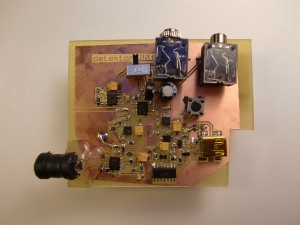
\includegraphics[width=.5\textwidth]{detektors}
	    \caption{The Detektor system, courtesy of detektor.org}
	\end{figure}

His \textit{Earthcodes} project attempts to boot computer off of telluric noise by planting part of the motherboard straight into soil \citep{whitelaw2013}. 

\begin{figure}[H]
	  \centering
	    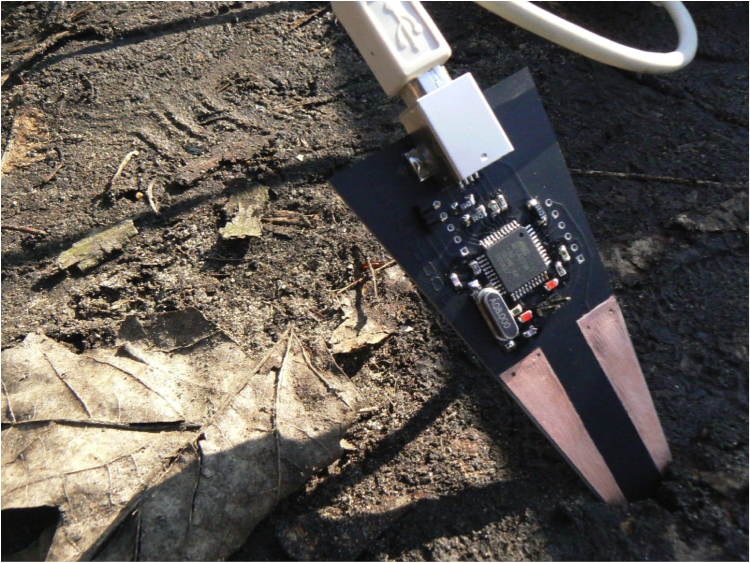
\includegraphics[width=1\textwidth]{earthcodes}
	     \caption{The Earthboot board, courtesy of \citep{whitelaw2013}}
	\end{figure}

Performances are extremely tactile and hybrid, blending digital electronics, analog electronics and organic matter. 

\begin{figure}[H]
	  \caption{Martin Howse performing with soil, chemicals, various electronics. Courtesy of Arté Télévision.}
	  \centering
	    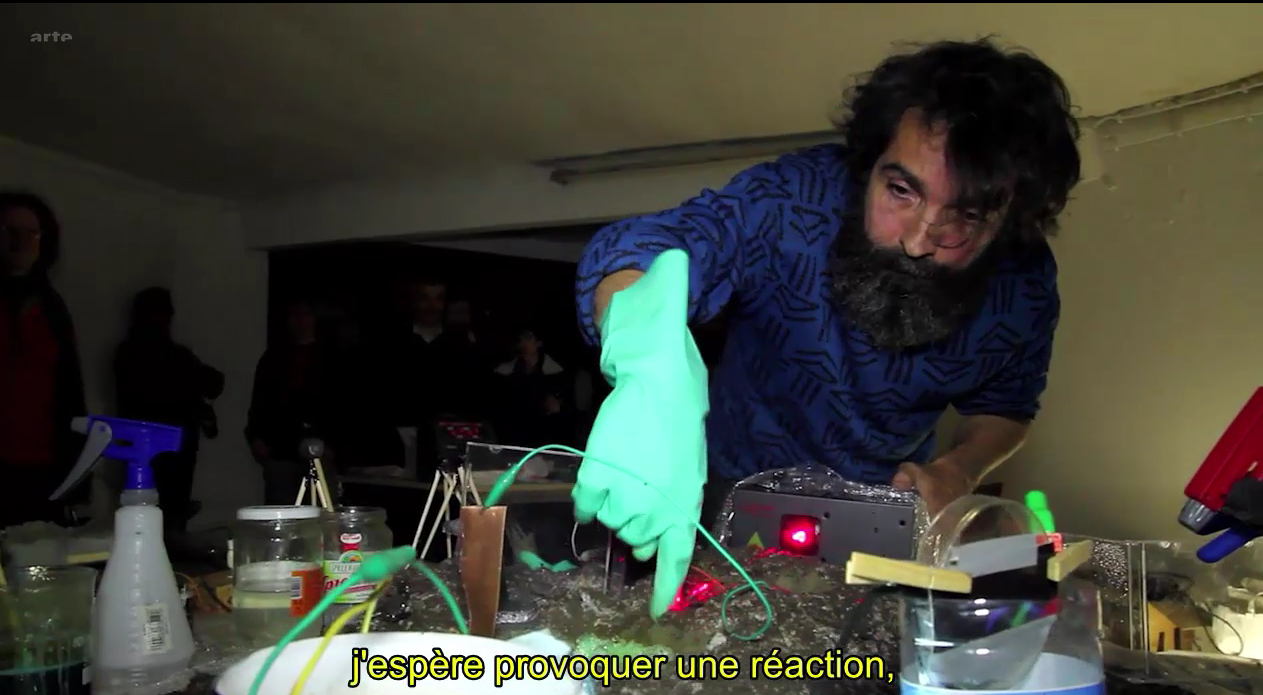
\includegraphics[width=1\textwidth]{howseperf}
	\end{figure}
	
He was interviewed in order to better appreciate the intentions behind some of these unusual design and performance practices, keeping in mind themes of post-optimality, levels of innovation in electronic music devices, and community.  

\begin{quote}
	I hardly ever use electronic instruments other than those I have built myself and some of these I have had huge problems in trying to reduce the complexity — this has been the hardest work, how to map a vast mind-set of connections and processes to a simple interface. Working with materials presents a simpler interface.
\end{quote}

His answer to problems of complex electronics is to go through a contact with raw materials, an approach particularly reminiscent of Perner-Wilson's \textit{Kit-of-No-Parts}. 

\begin{quote}
	the approach is very much a revealing, either through re-working materials towards technology (for example, performances using earth as an active, electrochemical, biologic material), or dissecting and almost dissolving (in chemical sense) digital technology (in workshops), or devising software which examines its own material conditions
\end{quote}

Post-optimality is omnipresent in Howse's work: at the component level, through the use of organic or soft, unstable materials such as soil, acids and fungus \citep{howse}. At the systems level, this is noticeable by his attempts to boot operating systems using noise as sections of code (the earthcode project) or his circuit combining turntable needle and FM radio. 

\begin{figure}[H]
	  \caption{The FM needle, a hybrid of turntable needle and FM transmitter. courtesy of 1010.co.uk}
	  \centering
	    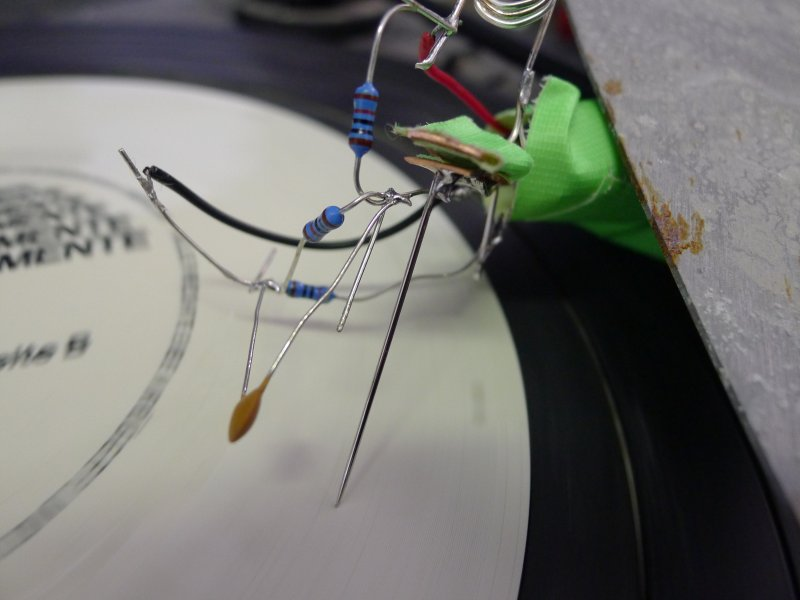
\includegraphics[width=1\textwidth]{howseFMneedle}
	\end{figure}
	
At the interface level, post-optimality is objectified in his irregular set of copper contacts in the dark interpreters series (see subsection 3.7.1). Their goal is to present a tangible surface for machine languages: ``I wanted the user to literally put their fingers into the code, to run the code over their skin'' 

In these processes, the importance of teaching as a method for inspiration and self-learning parallels the ideas discussed with Collins: these are projects he teaches in workshops, devices he sells, or are part of a performance routine. It is important to note Howse' unique background in literature, video art and teaching, which heavily permeates his technical practices: 

\begin{quote}
	 I began working mostly within video and conceptual art and realized that technology was an important material concern for me; teaching as in workshops is a way of generating new ideas for myself and others.
\end{quote}

Once again, post-optimal devices find a social dimension.
 
Howse's designs were previously qualified as both open source and cryptic, and this is relevant to a discussion of post-optimal design methods. Schematics, codes and poetic presentations of his work are all available online. All were developed using open source software. However, through his use of software such as KiCad (an open source and fully free alternative to professional computer circuit design software) and a personal set of code formatting rules, much of Howse's documentation offers a slight user-unfriendliness also described in section 3.7.1 which clearly encourage learning. This is done in a matter similar to that described by Kevin Ernste when discussing Cihan's \textit{Porcupine} device: provide just enough information to allow attempts at reproduction, but with enough uncertainty to prevent fully accurate duplication (see section 3.4.1).  

Collins and Rylan both expressed concerns with the difficulty of ``real'' engineering and the rarity of compelling performances from electronic music hardware makers. Howse appears to address both concerns: he is perhaps the best user of his own designs, but also seems successful enough with them to be making second runs of completed devices. Post-optimality permeates every single of his endeavors, hinting towards a tongue-in-cheek look at musical engineering that nevertheless must be contextualized with his wide-ranging technical skills.

\section{Sang Wook ``Sunny'' Nam and Joshua Florian}

Sunny and Josh both operate in a very niche market of ``highest-end'' audio. Their businesses are built upon a reputation for the absolute highest standards of performance, and their investment in such a reputation directly correlates with their continued success. Although a reader will find technical information in their interview transcripts, it seemed most important to include comments on their responses here because they address greater cultural contexts for some important concepts of audio technology in our discussion of open design. 

Effectively, Sunny and Josh are both secretive about the details of their work. As Sunny explains, he's spent countless hours and invested a significant amount of capital into designing a studio that is not only unique, but also objectively one of the best listening rooms in North America. In parallel, Josh's design for Sunny are entirely custom, fine-tuned affairs that they collaborate on to optimize until both of their standards for quality audio are satisfied.``The concepts are most important'', he'll say, explaining why he thinks product schematics shouldn't be made available in most cases. 

Their time spent together at the Mastering Lab in Los Angeles makes them share a similar language and respect for what they call ``yestertech'', a term coined by their supervisor there. In some interesting regards, this interest and respect is the cultural bridge between high end commercial audio and the concept of open design previous chapters experimentally defined. 

An informal definition of yestertech according to Josh and Sunny would probably follow these lines: a collection of devices and their associated designs and histories that were designed for the specific purposes of sounding as good as possible, often site or context specific, manufactured in small numbers if ever in mass, and often pre-dating the commercial boom of digital audio. In that sense, the golden years of yestertech surround the two two world wars, perhaps extending to the mid seventies. 

Going back to our historical description of making in electronic music, one might see a correlation between this period and the rise of kit-raised electronics engineers. This is largely confirmed by Josh's personal experience, as he describes his teachers being mostly from that generation and milieu. Those personalities came out of research institutions or large businesses (often aerospace, defense or both) and brought with them a academic and company cultures that largely subsides in todays major label recording and mastering world. That institutionalized vision of electric music largely fueled the development of the music industry until the eighties. 

Interestingly, Josh acknowledges that this model largely relied on a mentor-based system of information-sharing. Arguing that this is an inherently pre-internet practice is out of the scope of this thesis, however, denying the rise of self-taught experimenters following the Tudor model (aware of larger trends but faithful to self-contained aesthetic aspirations) would be short-sighted. 

Drawing a caricature, a first glance would offer a convenient spectrum of practices: on one end, the blissfully unaware of circuit theory bender and chaotic noise musician, and the professional, mentored, traditionalist engineer on the other. Their obvious and common interest in yestertech shows how inconsistent a classification of practitioners (let alone practices) would be if it followed this spectrum. Roland just announced its first series of eurorack modules\citep{factmag2015}, bringing the institution to a market founded and mostly kept alive by quirky revivalists (see appendix A-3 for a more in depth description of that evolution). Ray Wilson, online DIY synthesizer guru recently released a book on analog systems through Maker Media Inc., owned by major publisher O'Reilly media \citep{wilson2013}. Technological comebacks or extended lives as cultural phenomenas are at this point commonplace in audio (tube amps, analog synths, vinyl, cassettes, AlNiCo magnets...): yestertech is, if not half the game of audio equipment design, a binding point for most communities. 

Dan Snazelle, in describing his work as entirely original, is compelled to make a significant addendum: ``analog electronics are rarely entirely new''. In the current context, where chip-tune motivates people to make the most of intentionally limited 8 bit systems and bases entire synthesis schemes off of Commodore 64 SID ICs, it seems almost natural to extend yestertech to \emph{any pre-existing audio equipment that's existed long enough to see a few generations of production and hacking}, thereby maintaining the relevance of the term.

\section{Overview} 

 Various post-optimal practices have been identified at various levels of the electronics design and manufacturing chain. These practices recur explicitly in connection to the boundary between analog and digital technologies, and implicitly through an underlying connection to chaotic or unpredictable systems. Those systems are usually centered on electronics, except in Collins', Jones' and Howse's case where they also find an extended basis in the social aspects of their sound experiments through tutorials, classes and open documentation. Paraphrasing Joe Paradiso's statement that hacking is pervasive, post-optimality could be described as a latent characteristic of hardware-based musical practices.

